В текстах задач олимпиад Казахстанского филиала упоминаются студенты, которые активно участвовали в олимпиадном движении филиала в период с 2012 по 2017 год и, в частности, принимали участие в чемпионате мира по программированию ACM ICPC.

Чемпионат мира по программированию проводится в несколько этапов. Четвертьфинал чемпионата мира для команд из Казахстана проводится параллельно в Алматы и Астане в конце октября. Обычно он собирает около 100 команд, представляющих около 30 университетов Казахстана. Около 30 лучших команд (но не более 4 команд из одного университета) приглашаются на следующий этап --- полуфинал чемпионата мира.

Команды, отобранные на 16 четвертьфиналах Северо-Восточного Европейского региона, встречаются на полуфинале в начале декабря. Соревнование проводится параллельно на одном и том же наборе задач сразу на четырех площадках: Ташкент (до 2015 года), Алматы (с 2016 года), Барнаул, Тбилиси и Санкт-Петербург. Как правило, это около 240 команд, представляющие 120 ВУЗов данного региона. Около 15 лучших команд (но не более 1 команды из одного университета) приглашаются на финал.

Всего за 6 сезонов с 2012 по 2017 год в четвертьфинале команды представляли филиал 21 раз, из которых 17 раз успешно квалифицировались на полуфинал. Команда филиала принимала участие в полуфинале на трех разных площадках: г. Ташкент в 2012 году, г. Барнаул в 2013 и 2015 годах и г. Алматы в 2016 и в 2017 годах. Лучшим достижением команд филиала на полуфинале является дипломы Средней Азии (г. Ташкент, 2012), Сибири (г. Барнаул, 2015), Северо-Восточного Европейского региона (г. Алматы, 2016).

Команды филиала состоят из студентов, обучающихся по направлениям <<Математика>> и <<Прикладная математика>>. Многие участники команд филиала знакомятся с олимпиадами по програмированию в течении первого года обучения. Уже ко второму курсу они часто выступают на равных с опытными соперниками из других ВУЗов Казахстана.

Условия задач, результаты и материалы четвертьфиналов и полуфинала чемпионата мира по программированию ACM ICPC доступны на официальном сайте организатора в лице Санкт-Петербургского национального исследовательского университета информационных технологий, механики и оптики: https://neerc.ifmo.ru.

\subsubsection*{2012--2013 учебный год}

\paragraph{Четвертьфинал чемпионата (Казахстан).} Казахстанский филиал МГУ занял 6 место из 28 ВУЗов Казахстана, а лучшая команда филиала --- 22 место из 110 команд.

\paragraph{Полуфинал чемпионата (Средняя Азии).} Казахстанский филиал МГУ занял 11 место из 18 ВУЗов Средней Азии, а лучшая команда филиала --- 22 место из 47 команд Средней Азии (15 место из 29 среди команд из Казахстана). Данный результат отмечен \textbf{дипломом третьей степени среди команд Казахстана}.

\paragraph{Полуфинал чемпионата (СНГ).} Казахстанский филиал МГУ занял 92 место из 129 ВУЗов СНГ, а лучшая команда филиала --- 153 место из 229 команд. Данный результат отмечен \textbf{дипломом третьей степени среди команд Средней Азии}. К слову, команды МГУ заняли 2, 6, 7, 9 и 10 места.

\begin{center}
\begin{tabular}{|p{1.8cm}|p{5.5cm}|p{1.5cm}|p{1.6cm}|l|}
\hline
Команда & Состав & 1/4 \newline Астана & 1/2 \newline Ташкент\\
\hline
Jusual &
Максимец Илья, ВМ-4, \newline
Суворова Юлия, ММ-2, \newline
Жадиков Дамир, ММ-1. 
&
22 место \newline
4 задачи
&
22 место \newline
2 задачи
\\
\hline
\end{tabular}
\end{center}

\newpage
\begin{center}
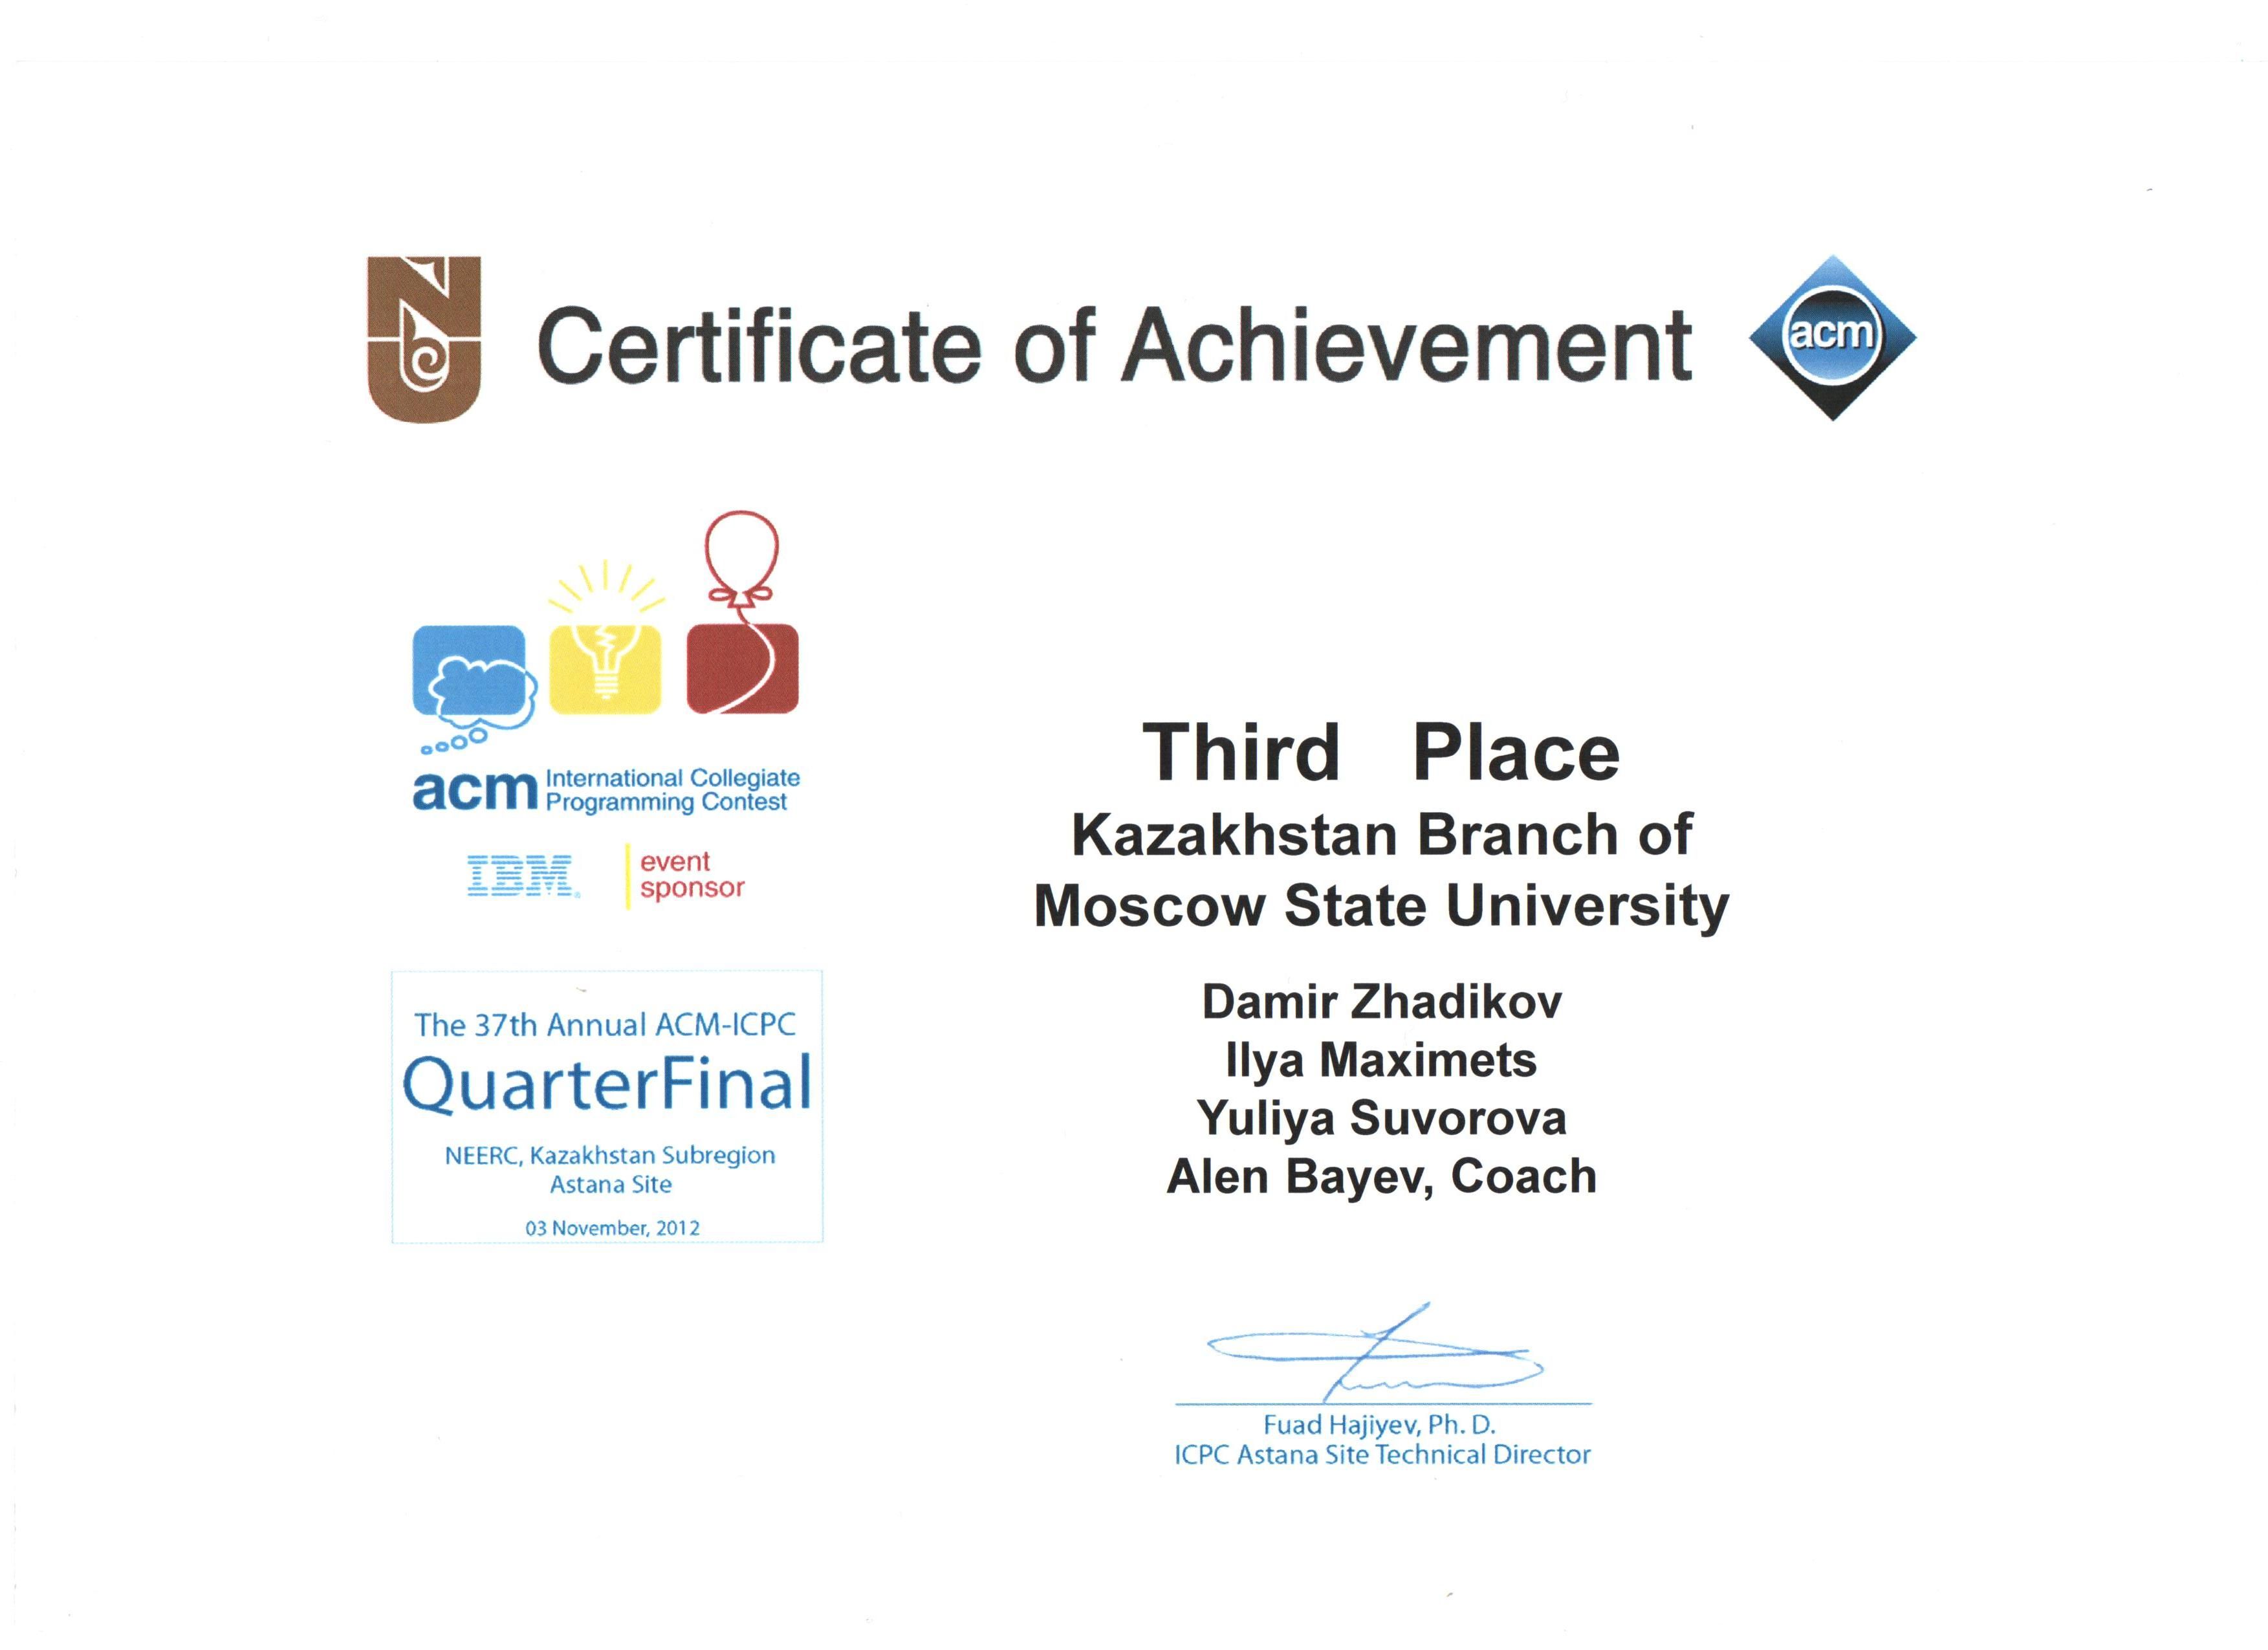
\includegraphics[width=0.7\linewidth]{diploma/2012-astana}

Диплом 3 степени среди команд Казахстана 2012\\
Команда Jusual (Максимец, Суворова, Жадиков).
\end{center}

\begin{center}
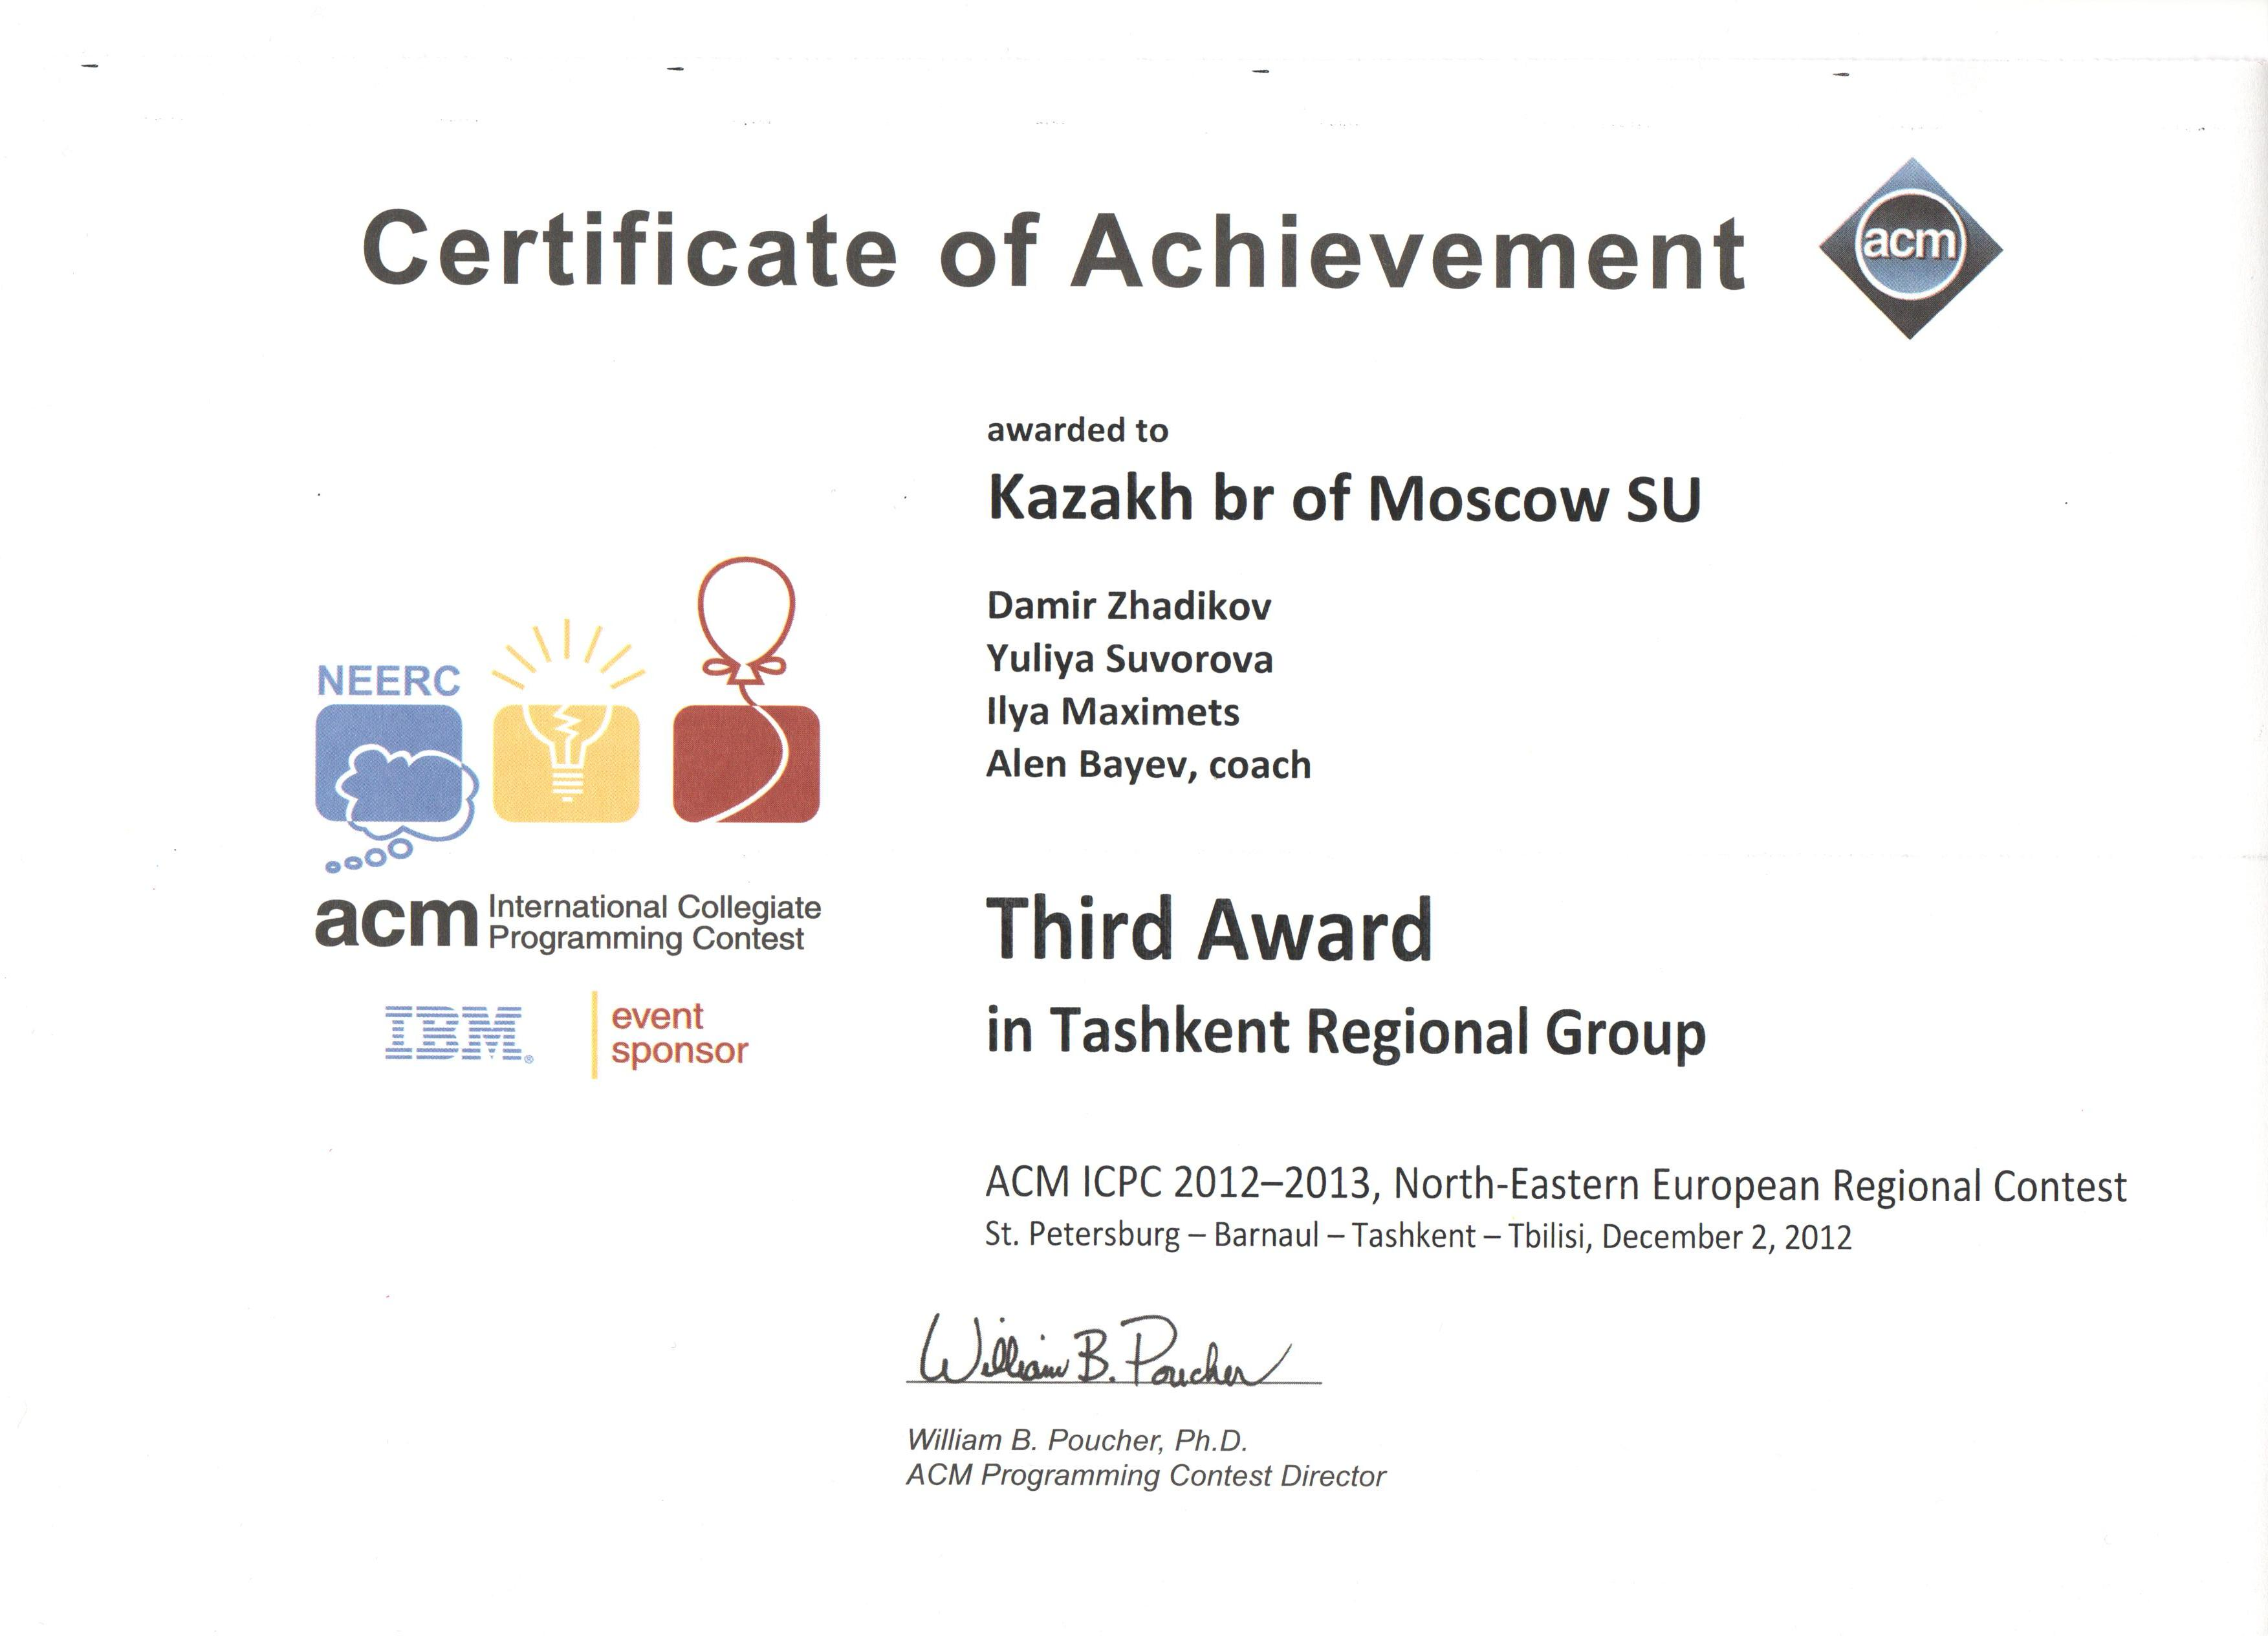
\includegraphics[width=0.7\linewidth]{diploma/2012-tashkent}

Диплом 3 степени среди команд Центральной Азии 2012\\
Команда Jusual (Максимец, Суворова, Жадиков).
\end{center}
\newpage

\subsubsection*{2013--2014 учебный год}

\paragraph{Четвертьфинал чемпионата (Казахстан).} Казахстанский филиал МГУ занял 10 место из 40 ВУЗов Казахстана, а лучшая команда филиала --- 29 место из 91 команды. Данный результат отмечен \textbf{дипломом в номинации <<Лучшая гостевая команда на площадке в Астане>>}.

\paragraph{Полуфинал чемпионата (Сибирь).} Казахстанский филиал МГУ занял 17 место из 29 ВУЗов Сибири, а лучшая команда филиала --- 25 место из 44 команд Сибири (17 место из 30 среди команд из Казахстана).

\paragraph{Полуфинал чемпионата (СНГ).} Казахстанский филиал МГУ занял 78 место из 117 ВУЗов СНГ, а лучшая команда филиала --- 147 место из 228 команд. К слову, команды МГУ заняли 2, 10, 11, 12, 27 места.

\begin{center}
\begin{tabular}{|p{1.8cm}|p{5.5cm}|p{1.5cm}|p{1.6cm}|l|}
\hline
Команда & Состав & 1/4 \newline Астана & 1/2 \newline Барнаул \\
\hline
Big dipper &
Тлеубаев Адиль, ВМ-2, \newline
Таранов Денис, ВМ-1, \newline
Шокетаева Надира, ММ-1. 
&
29 место \newline
5 задач
&
25 место \newline
2 задачи
\\
\hline
Lord \newline Bendtner \newline Team &
Седякин Илья, ВМ-1, \newline
Таскынов Ануар, ВМ-1, \newline
Васильев Андрей, ВМ-1. 
&
46 место \newline
4 задачи
&
-
\\
\hline
\end{tabular}
\end{center}

\newpage
\mbox{}
\vfill
\begin{center}
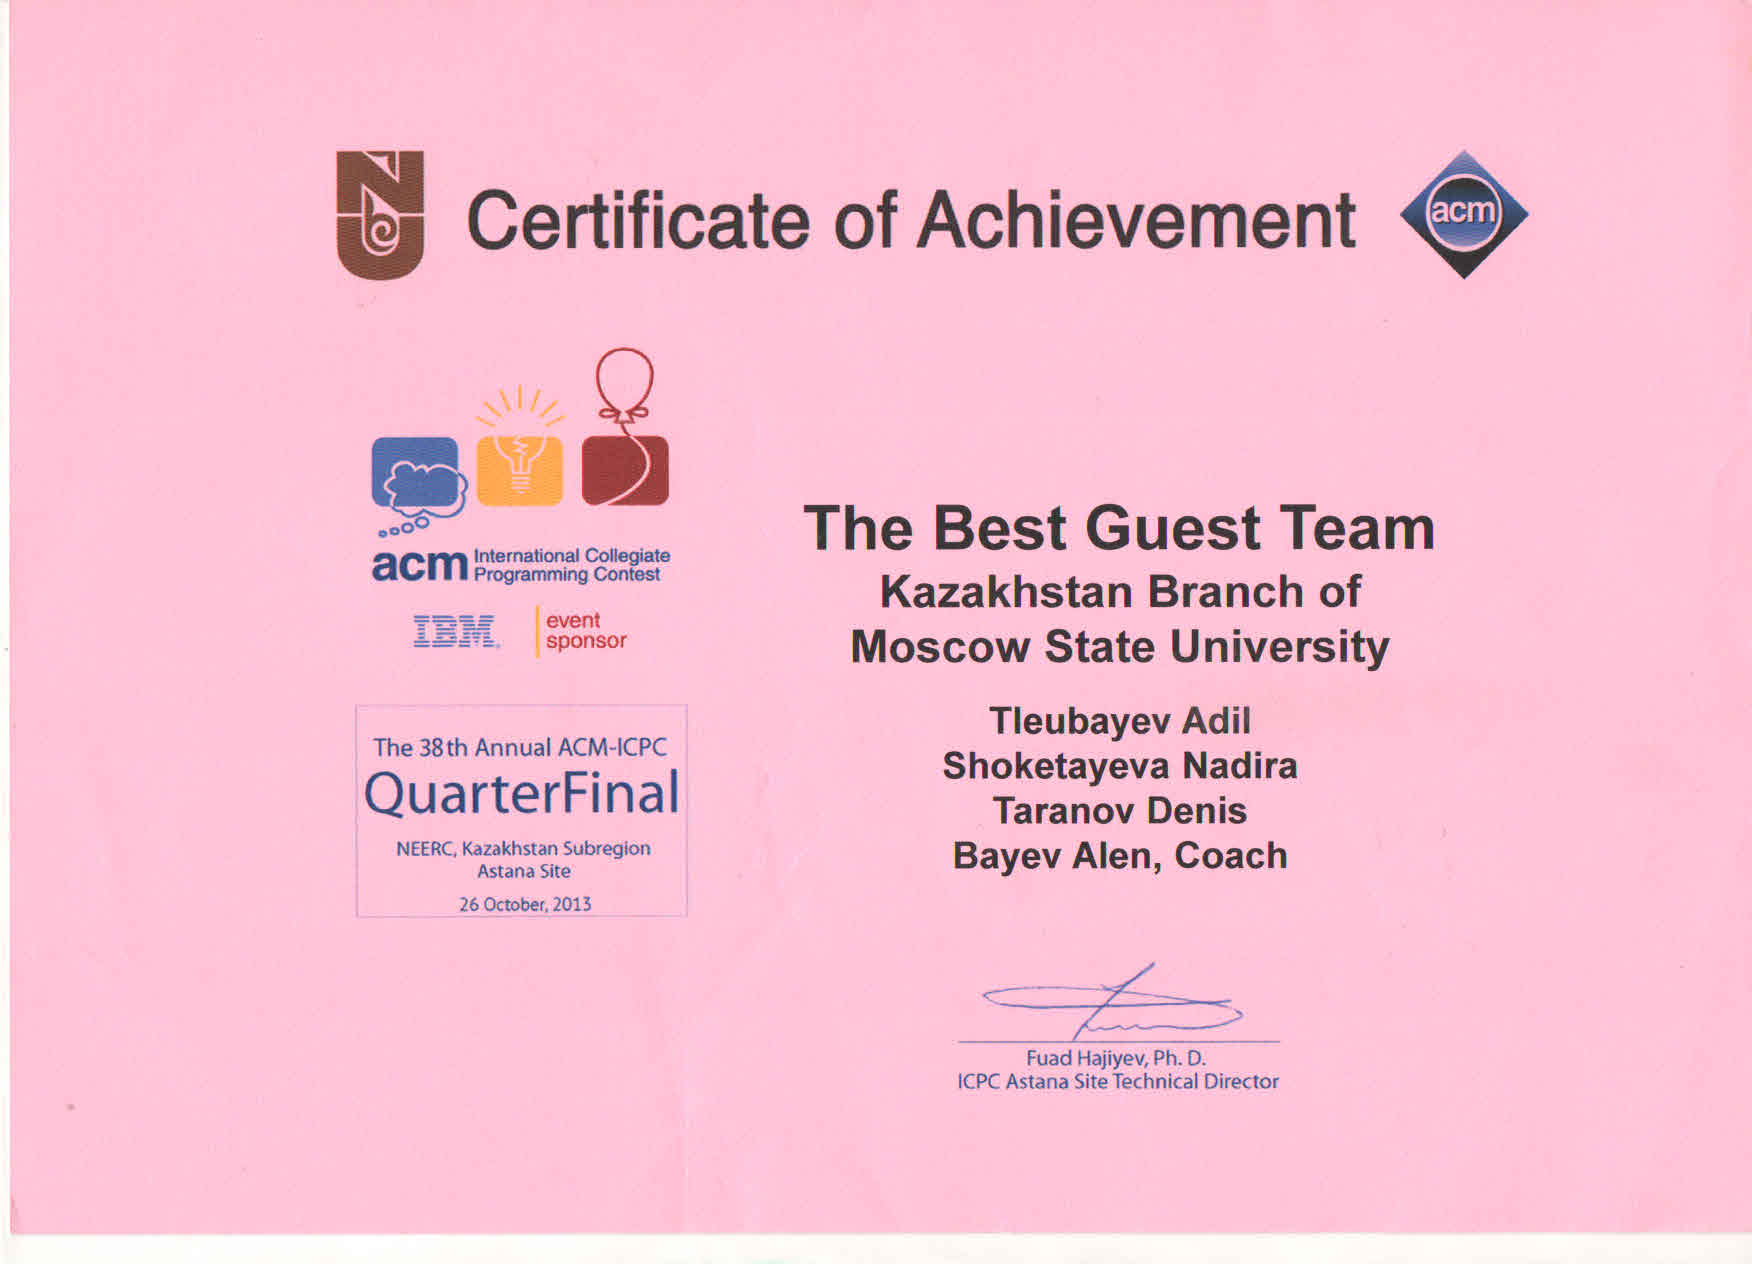
\includegraphics[width=0.8\linewidth]{diploma/2013-astana}

Диплом в номинации <<Лучшая гостевая команда на площадке в Астане>>

Команда Big dipper (Тлеубаев, Таранов, Шокетаева).
\end{center}
\vfill
\mbox{}
\newpage
\subsubsection*{2014--2015 учебный год}

\paragraph{Четвертьфинал чемпионата (Казахстан).} Казахстанский филиал МГУ занял 8 место из 30 ВУЗов Казахстана, а лучшая команда филиала --- 24 место из 98 команды.

\begin{center}
\begin{tabular}{|p{1.8cm}|p{5.5cm}|p{1.5cm}|p{1.6cm}|l|}
\hline
Команда & Состав & 1/4 \newline Астана & 1/2 \newline Барнаул\\
\hline
Lord \newline Bendtner \newline Team &
Седякин Илья, ВМ-2, \newline
Таскынов Ануар, ВМ-2, \newline
Вержбицкий Владислав, ВМ-2. 
&
24 место \newline
4 задачи
&
-
\\
\hline
MSU 4 &
Амир Мирас, ВМ-2 \newline
Шабхатов Асылжан, ВМ-2 \newline
Токтаганов Адиль, ММ-2 &
39 место \newline
3 задачи
&
-
\\
\hline
Snowy \newline Cube &
Журавская Александра, ВМ-1 \newline
Камалбеков Тимур, ВМ-1 \newline
Абайулы Ерулан, ВМ-1
&
42 место \newline
2 задачи
&
x
\\
\hline
Big \newline Dipper &
Таранов Денис, ВМ-2 \newline
Шокетаева Надира, ММ-2 \newline
Жусупов Али, ММ-1
&
44 место \newline
2 задачи
&
x
\\
\hline
\end{tabular}
\end{center}

\newpage

\subsubsection*{2015--2016 учебный год}

\paragraph{Четвертьфинал чемпионата (Казахстан).} Казахстанский филиал МГУ занял 6 место из 15 ВУЗов Казахстана, а лучшая команда филиала --- 23 место из 78 команд.

\paragraph{Полуфинал чемпионата (Сибирь).} Казахстанский филиал МГУ занял 12 место из 29 ВУЗов Сибири, а лучшая команда филиала --- 17 место из 44 команд Сибири (14 место из 16 среди команд из Казахстана).

\paragraph{Полуфинал чемпионата (СНГ).} Казахстанский филиал МГУ занял 70 место из 122 ВУЗов СНГ, а лучшая команда филиала --- 129 место из 224 команд. Данный результат отмечен дипломом третьей степени среди команд Сибири. К слову, команды МГУ заняли 4, 8, 65 и 68 места.

\begin{center}
\begin{tabular}{|p{1.8cm}|p{5.5cm}|p{1.5cm}|p{1.6cm}|l|}
\hline
Команда & Состав & 1/4 \newline Астана & 1/2 \newline Барнаул\\
\hline
Snowy \newline Cube &
Журавская Александра, ВМ-2 \newline
Камалбеков Тимур, ВМ-2 \newline
Абайулы Ерулан, ВМ-2
&
23 место \newline
6 задач
&
17 место \newline
3 задачи
\\
\hline
Big \newline Dipper &
Тлеубаев Адиль, ВМ-4, \newline
Таранов Денис, ВМ-3, \newline
Шокетаева Надира, ММ-3. 
&
25 место \newline
6 задач
&
-
\\
\hline
Lord \newline Bendtner \newline Team &
Седякин Илья, ВМ-3, \newline
Таскынов Ануар, ВМ-3, \newline
Вержбицкий Владислав, ВМ-3 
&
29 место \newline
5 задач
&
-
\\
\hline
Die \newline Perdimus &
Жусупов Али, ММ-2 \newline 
Турганбаев Сатбек, ВМ-2 \newline
Омаров Темирхан, ВМ-2
&
37 место \newline
4 задачи
&
-
\\
\hline
\end{tabular}
\end{center}

\newpage
\mbox{}
\vfill
\begin{center}
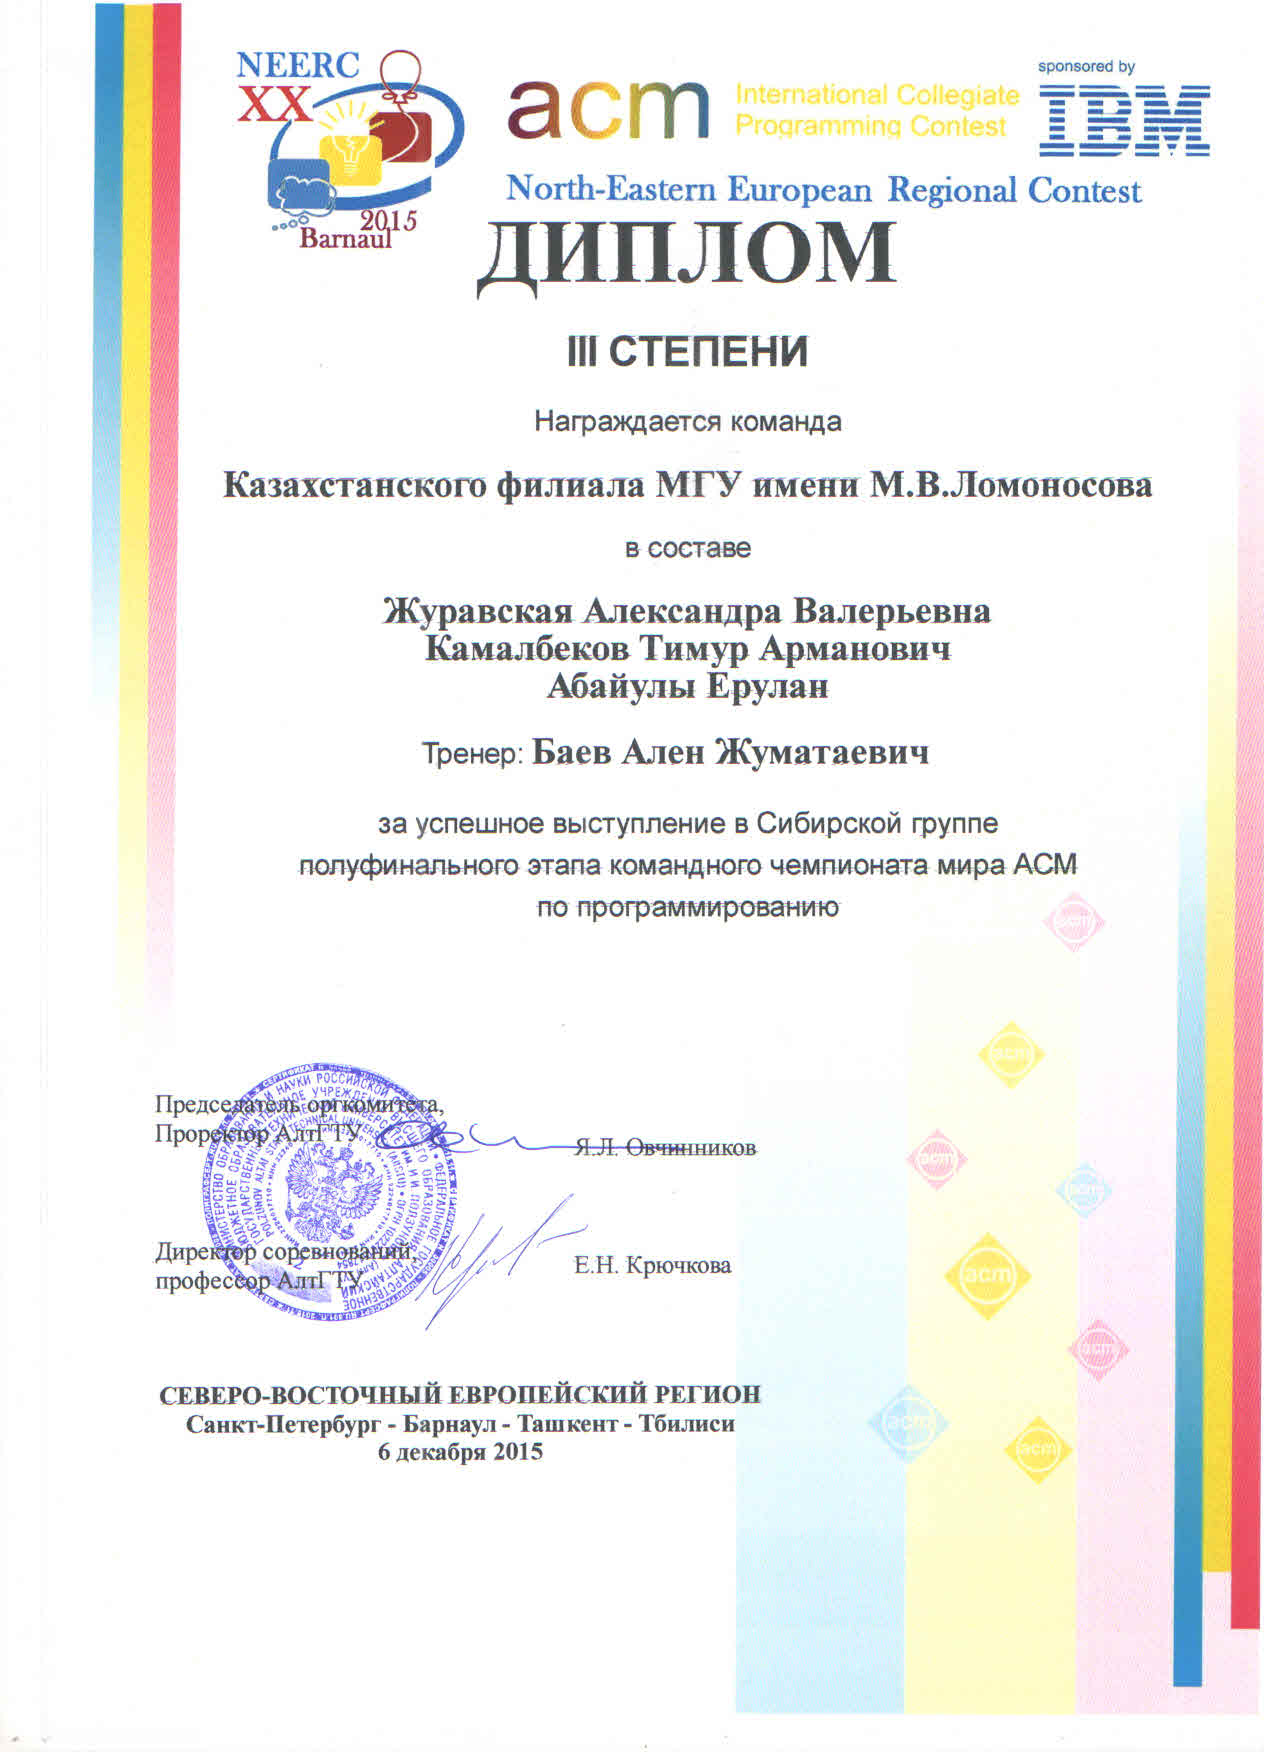
\includegraphics[width=0.8\linewidth]{diploma/2015-barnaul}

Диплом 3 степени среди команд Сибири 2015

Команда Snowy Cube (Журавская, Камалбеков, Абайулы).
\end{center}
\vfill
\mbox{}
\newpage



\subsubsection*{2016--2017 учебный год}

\paragraph{Четвертьфинал чемпионата (Казахстан).} Казахстанский филиал МГУ занял 7 место из 29 ВУЗов Казахстана, а лучшая команда филиала --- 20 место из 141 команды.

\paragraph{Полуфинал чемпионата (Средняя Азия).} Казахстанский филиал МГУ занял 5 место из 16 ВУЗов Средней Азии, а лучшая команда филиала --- 9 место из 42 команд Средней Азии (8 место из 28 среди команд из Казахстана). 

\paragraph{Полуфинал чемпионата (СНГ).} Казахстанский филиал МГУ занял 49 место из 109 ВУЗов СНГ, а лучшая команда филиала --- 93 место из 228 команд. Данный результат отмечен \textbf{дипломом третьей степени среди команд СНГ}. К слову, команды МГУ заняли 25, 27 и 72 места.

\begin{center}
\begin{tabular}{|p{2.0cm}|p{5.8cm}|p{1.5cm}|p{1.6cm}|l|}
\hline
Команда & Состав & 1/4 \newline Астана & 1/2 \newline Алматы\\
\hline
Snowy \newline Cube &
Журавская Александра, ВМ-3 \newline
Камалбеков Тимур, ВМ-3 \newline
Абайулы Ерулан, ВМ-3
&
20 место \newline
4 задачи
&
9 место \newline
3 задачи
\\
\hline
Big \newline Dipper &
Тлеубаев Адиль, ВМ-м, \newline
Амир Мирас, ВМ-4, \newline
Шокетаева Надира, ММ-4. 
&
38 место \newline
3 задачи
&
-
\\
\hline
Lord \newline Bendtner \newline Team &
Седякин Илья, ВМ-4, \newline
Таскынов Ануар, ВМ-4, \newline
Вержбицкий Владислав, ВМ-4
&
51 место \newline
3 задачи
&
-
\\
\hline
Nerzhul &
Болотников Димитрий, ММ-2 \newline
Газизов Куат, ММ-2 \newline
Аскергали Ануар, ВМ-1
&
52 место \newline
3 задачи
&
-
\\
\hline
Esprit &
Сеилов Айтмухаммед, ММ-2 \newline
Шарипов Азат, ВМ-1 \newline
Танкибаев Салима, ВМ-1
&
53 место \newline
3 задачи
&
x
\\
\hline
Complicate &
Коробов Павел, ММ-2 \newline
Бекмаганбектов Бекарыс, ММ-1 \newline
Кунакбаев Рамазан, ММ-1
&
69 место \newline
2 задачи
&
x
\\
\hline
\end{tabular}
\end{center}

\newpage
\mbox{}
\vfill
\begin{center}
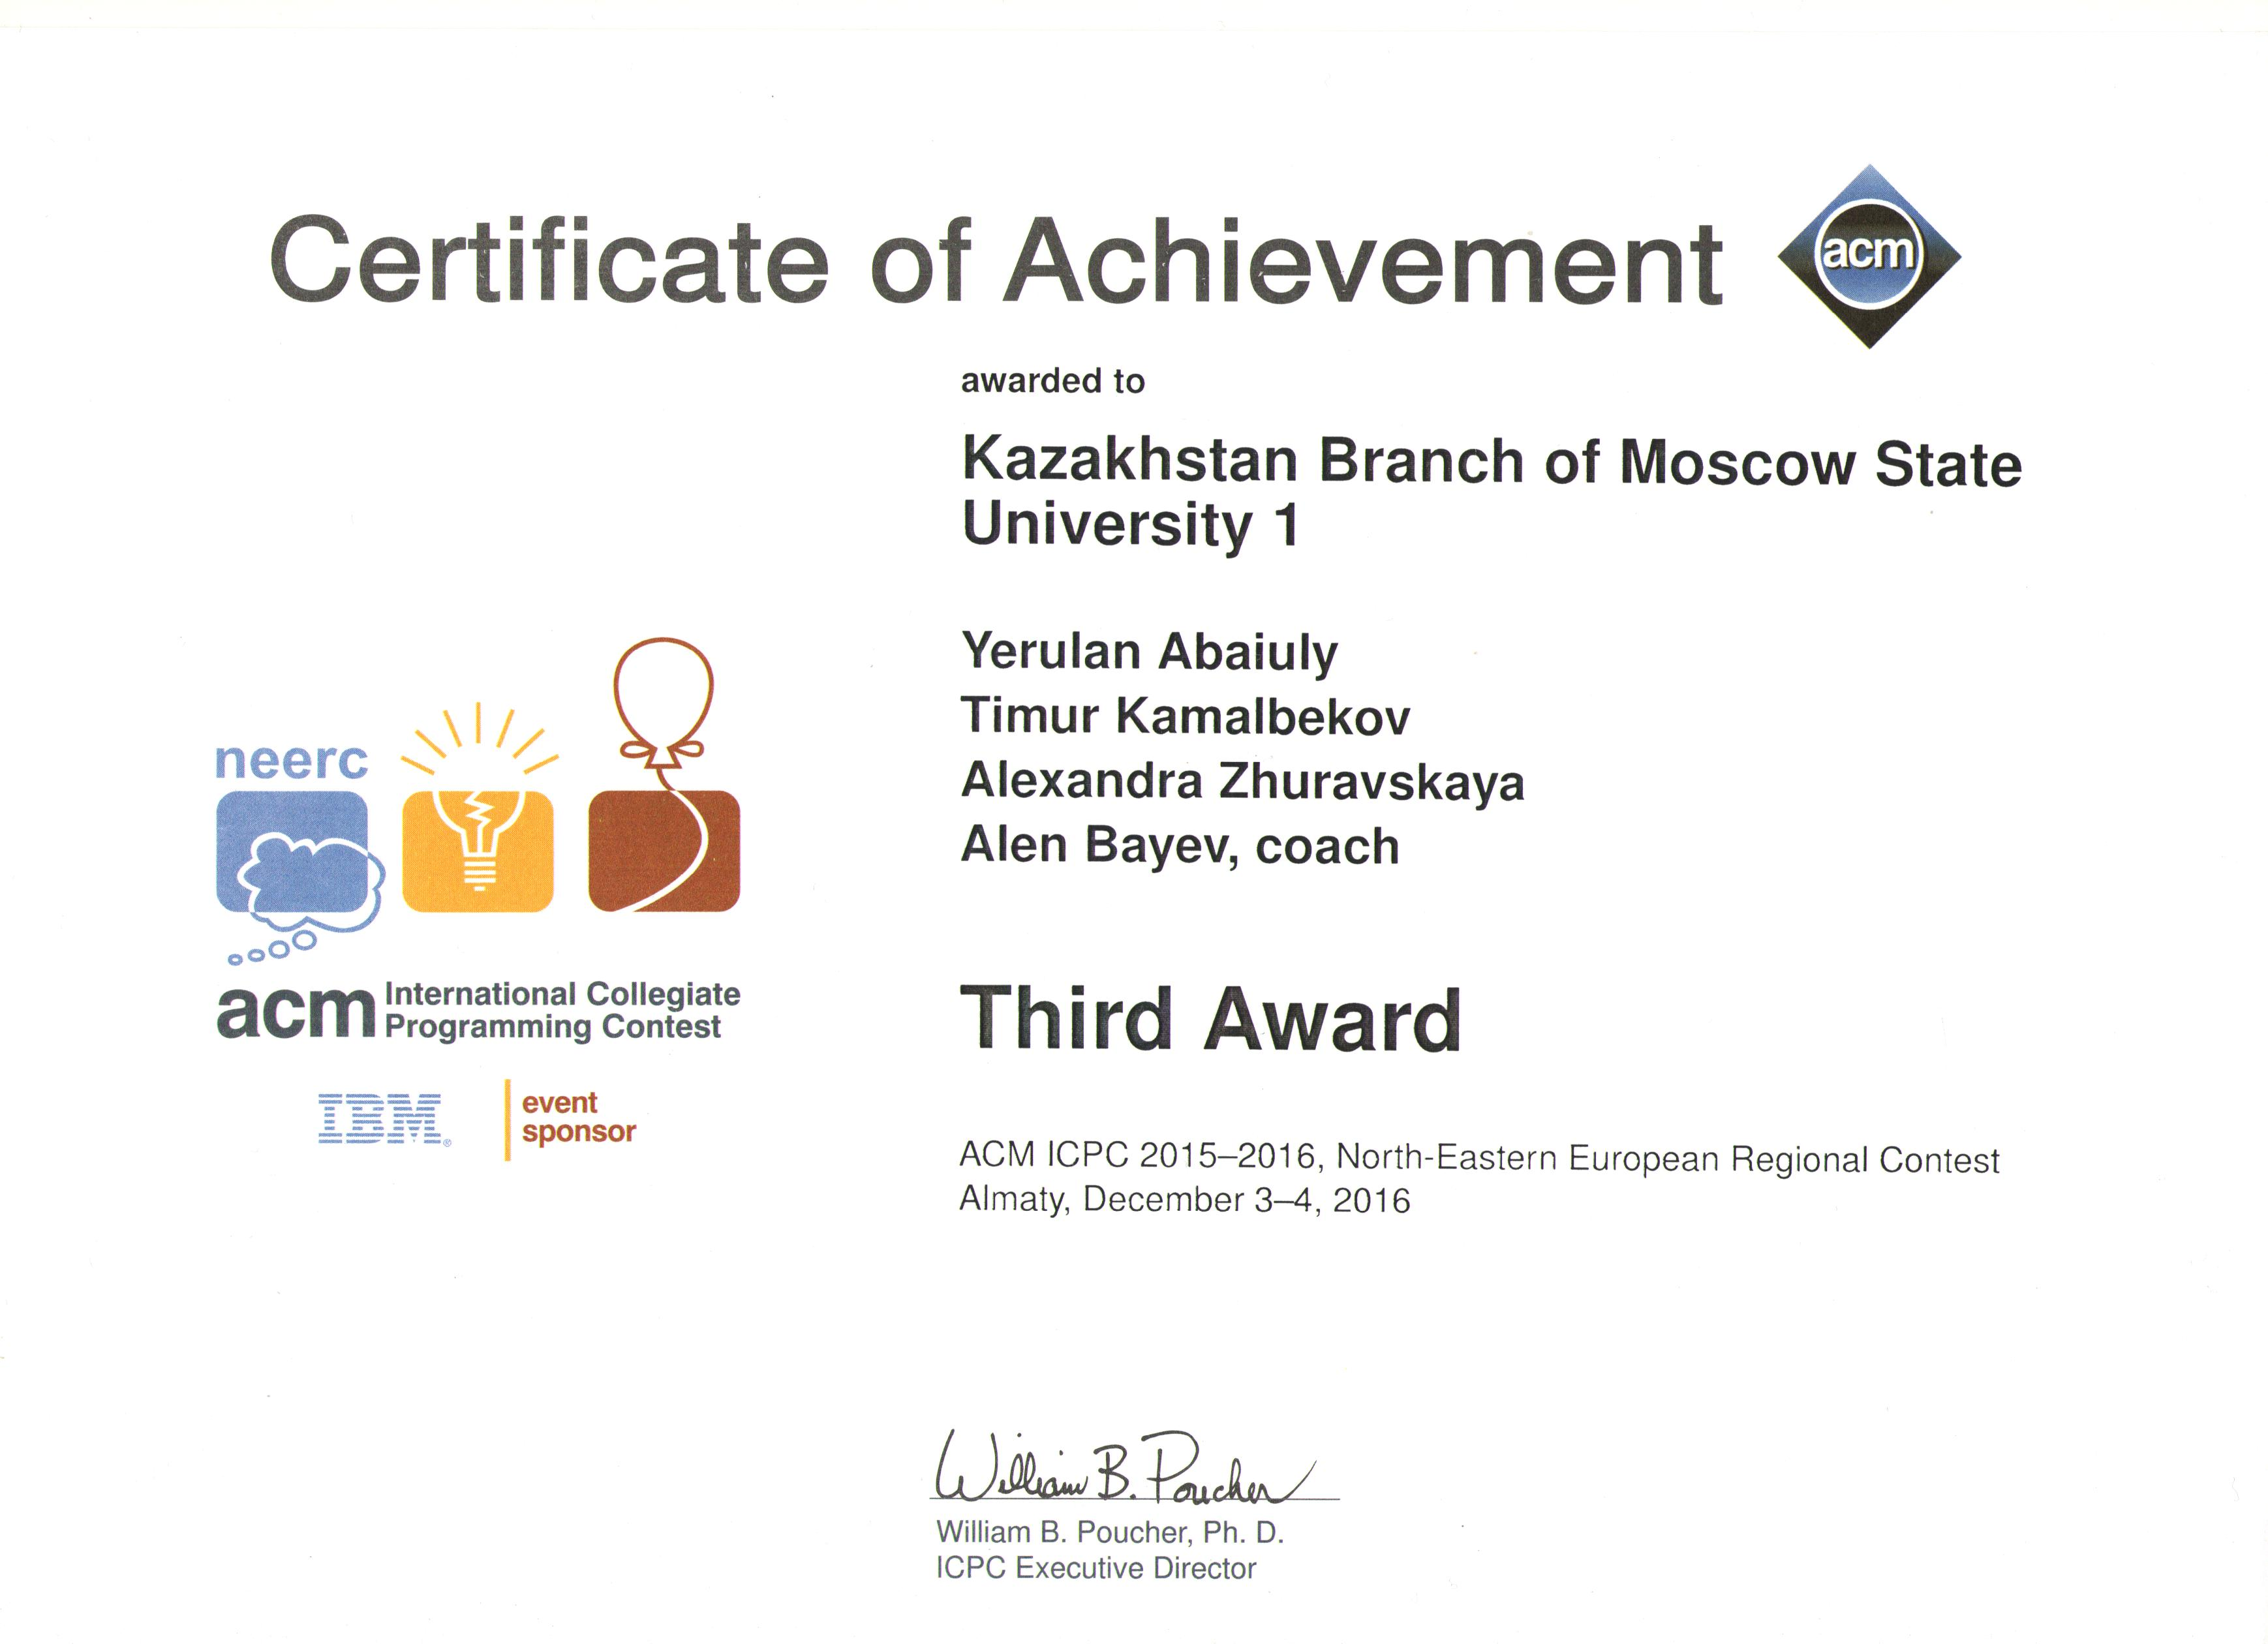
\includegraphics[width=0.9\linewidth]{diploma/2016-almaty}

Диплом 3 степени среди команд Северо-Восточного европейского региона (СНГ).

Команда Snowy Cube (Журавская, Камалбеков, Абайулы).
\end{center}
\vfill
\mbox{}
\newpage

\subsubsection*{2017--2018 учебный год}

\paragraph{Одна восьмая чемпионата (Москва).} Команда Snowy Cube участвовала в Московской ветке от МГУ. Заняла 40 место из 301 команды (11 место среди 29 команд МГУ). Данный результат отмечен \textbf{дипломом победителей одной восьмой финала в г. Москве}.

\paragraph{Четвертьфинал чемпионата (Москва).} Команда Snowy Cube заняла 48 место из 87 команды (11 место среди 12 команд МГУ).

\begin{center}
\begin{tabular}{|p{1.8cm}|p{5.8cm}|p{1.5cm}|p{1.6cm}|l|}
\hline
Команда & Состав & 1/8 \newline Москва & 1/4 \newline Москва \\
\hline
Brain \newline Burst &
Камалбеков Тимур, ВМК-4 \newline
Журавская Александра, ВМК-4 \newline
Абайулы Ерулан, ВМК-4 
&
40 место \newline
8 задач
&
48 место \newline
3 задачи
\\
\hline
\end{tabular}
\end{center}

\newpage
\mbox{}
\vfill
\begin{center}
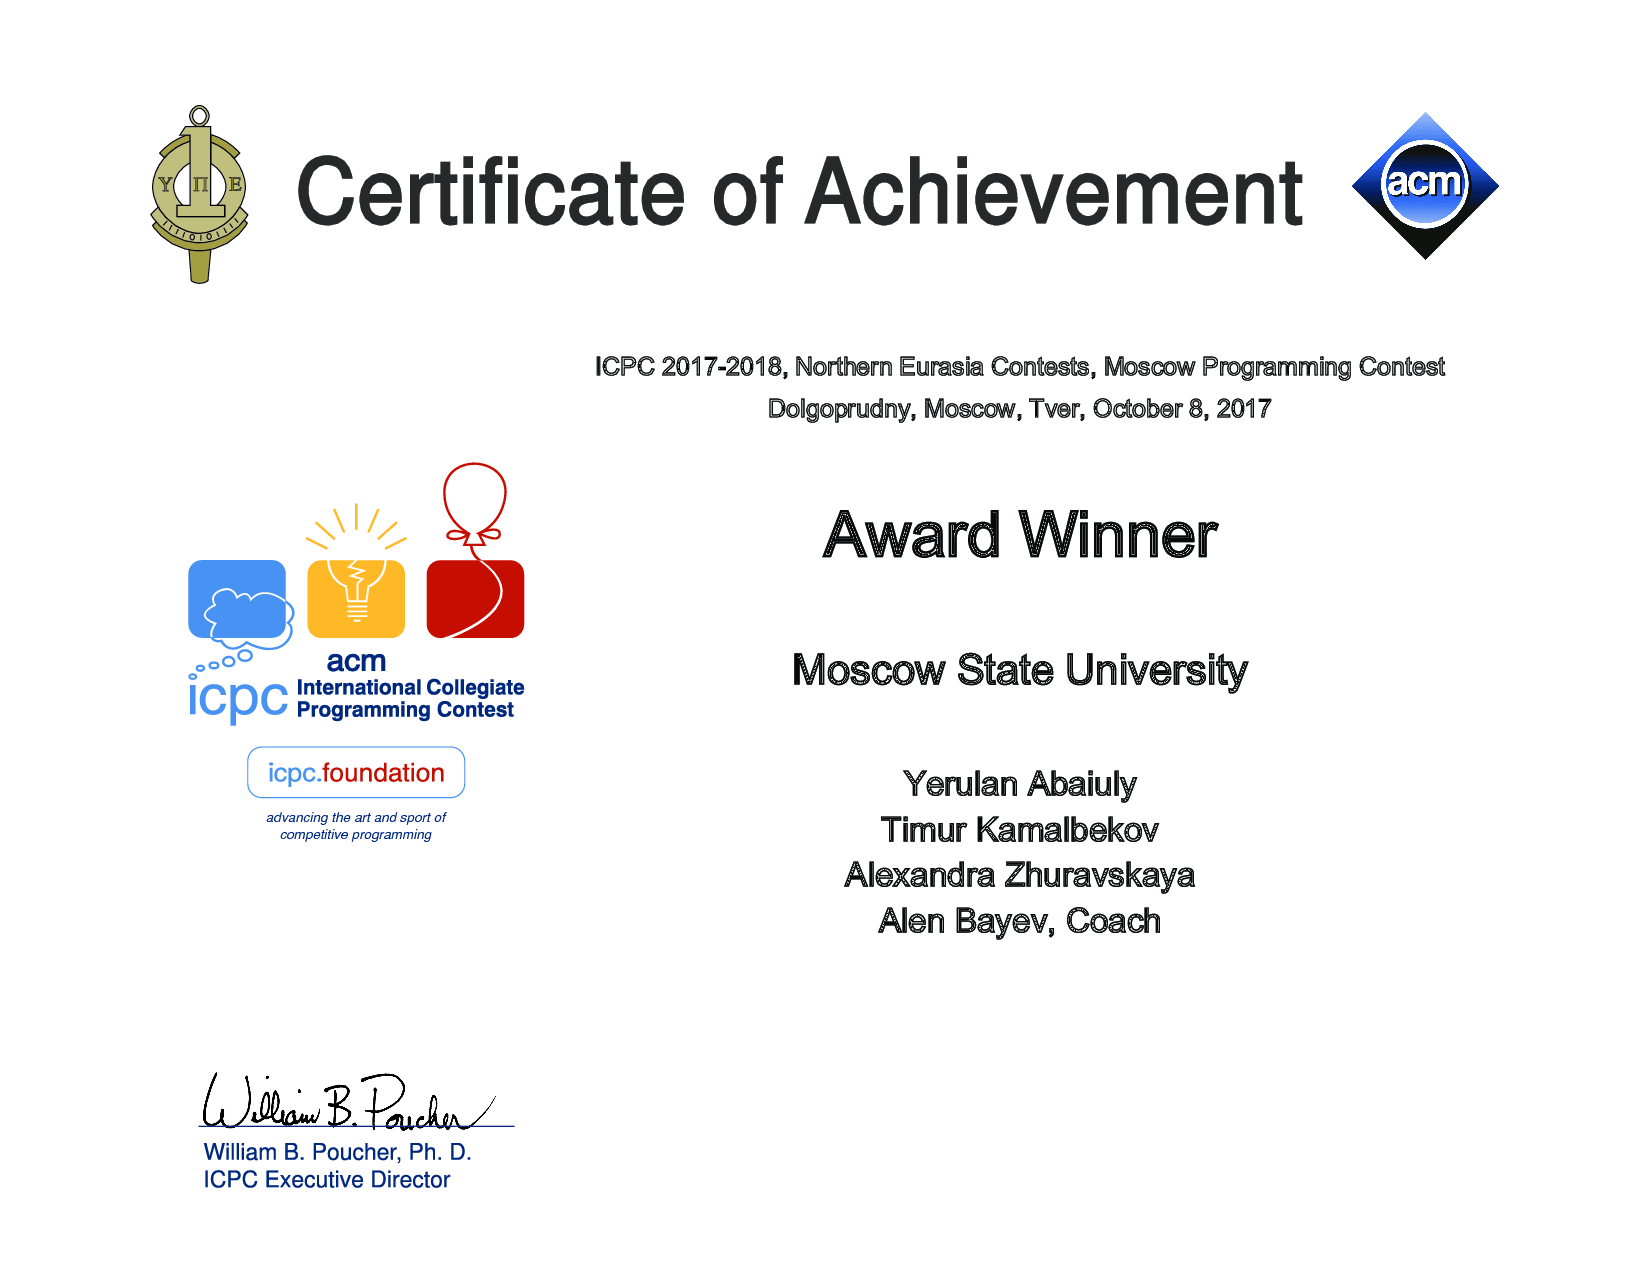
\includegraphics[width=0.9\linewidth]{diploma/2017-moscow}

Диплом победителей среди команд Москвы.

Команда Snowy Cube (Журавская, Камалбеков, Абайулы).
\end{center}
\vfill
\mbox{}
\newpage

\paragraph{Четвертьфинал чемпионата (Казахстан).} Казахстанский филиал МГУ занял 6 место из 14 ВУЗов Казахстана, а лучшая команда филиала --- 14 место из 122 команды.

\paragraph{Полуфинал чемпионата (Средняя Азия).} Казахстанский филиал МГУ занял 7 место из 45 ВУЗов Средней Азии, а лучшая команда филиала --- 10 место из 54 команд Средней Азии (6 место из 34 среди команд из Казахстана).

\paragraph{Полуфинал чемпионата (СНГ).} Казахстанский филиал МГУ занял 63 место из 126 ВУЗов СНГ, а лучшая команда филиала --- 127 место из 266 команд. К слову, команды МГУ заняли 2, 23, 30 и 40 места.

\begin{center}
\begin{tabular}{|p{2cm}|p{5.8cm}|p{1.5cm}|p{1.6cm}|l|}
\hline
Команда & Состав & 1/4 \newline Астана & 1/2 \newline Алматы\\
\hline
Brain \newline Burst &
Аскергали Ануар, ВМК-2 \newline
Бекмаганбетов Бекарыс, ММ-2 \newline
Шарипов Азат, ВМК-2 \newline
&
14 место \newline
7 задач
&
10 место \newline
3 задачи
\\
\hline
MSU 2 &
Кунакбаев Рамазан, ММ-2 \newline
Макатова Батима, ММ-2 \newline
Ержанов Жалгас, ВМК-2
&
25 место \newline
5 задач
&
-
\\
\hline
Murmaider &
Вагнер Алан, ВМК-1 \newline
Азатов Таир, ВМК-1 \newline
Понамарев Валерий, ВМК-1
&
30 место \newline
4 задачи
&
-
\\
\hline
Witty \newline name &
Газизов Куат, ММ-3 \newline
Болотников Димитрий, ММ-3 \newline
Коробов Павел, ММ-3 \newline
&
32 место \newline
4 задачи
&
-
\\
\hline
\end{tabular}
\end{center}

\newpage
\mbox{}
\vfill
\begin{center}
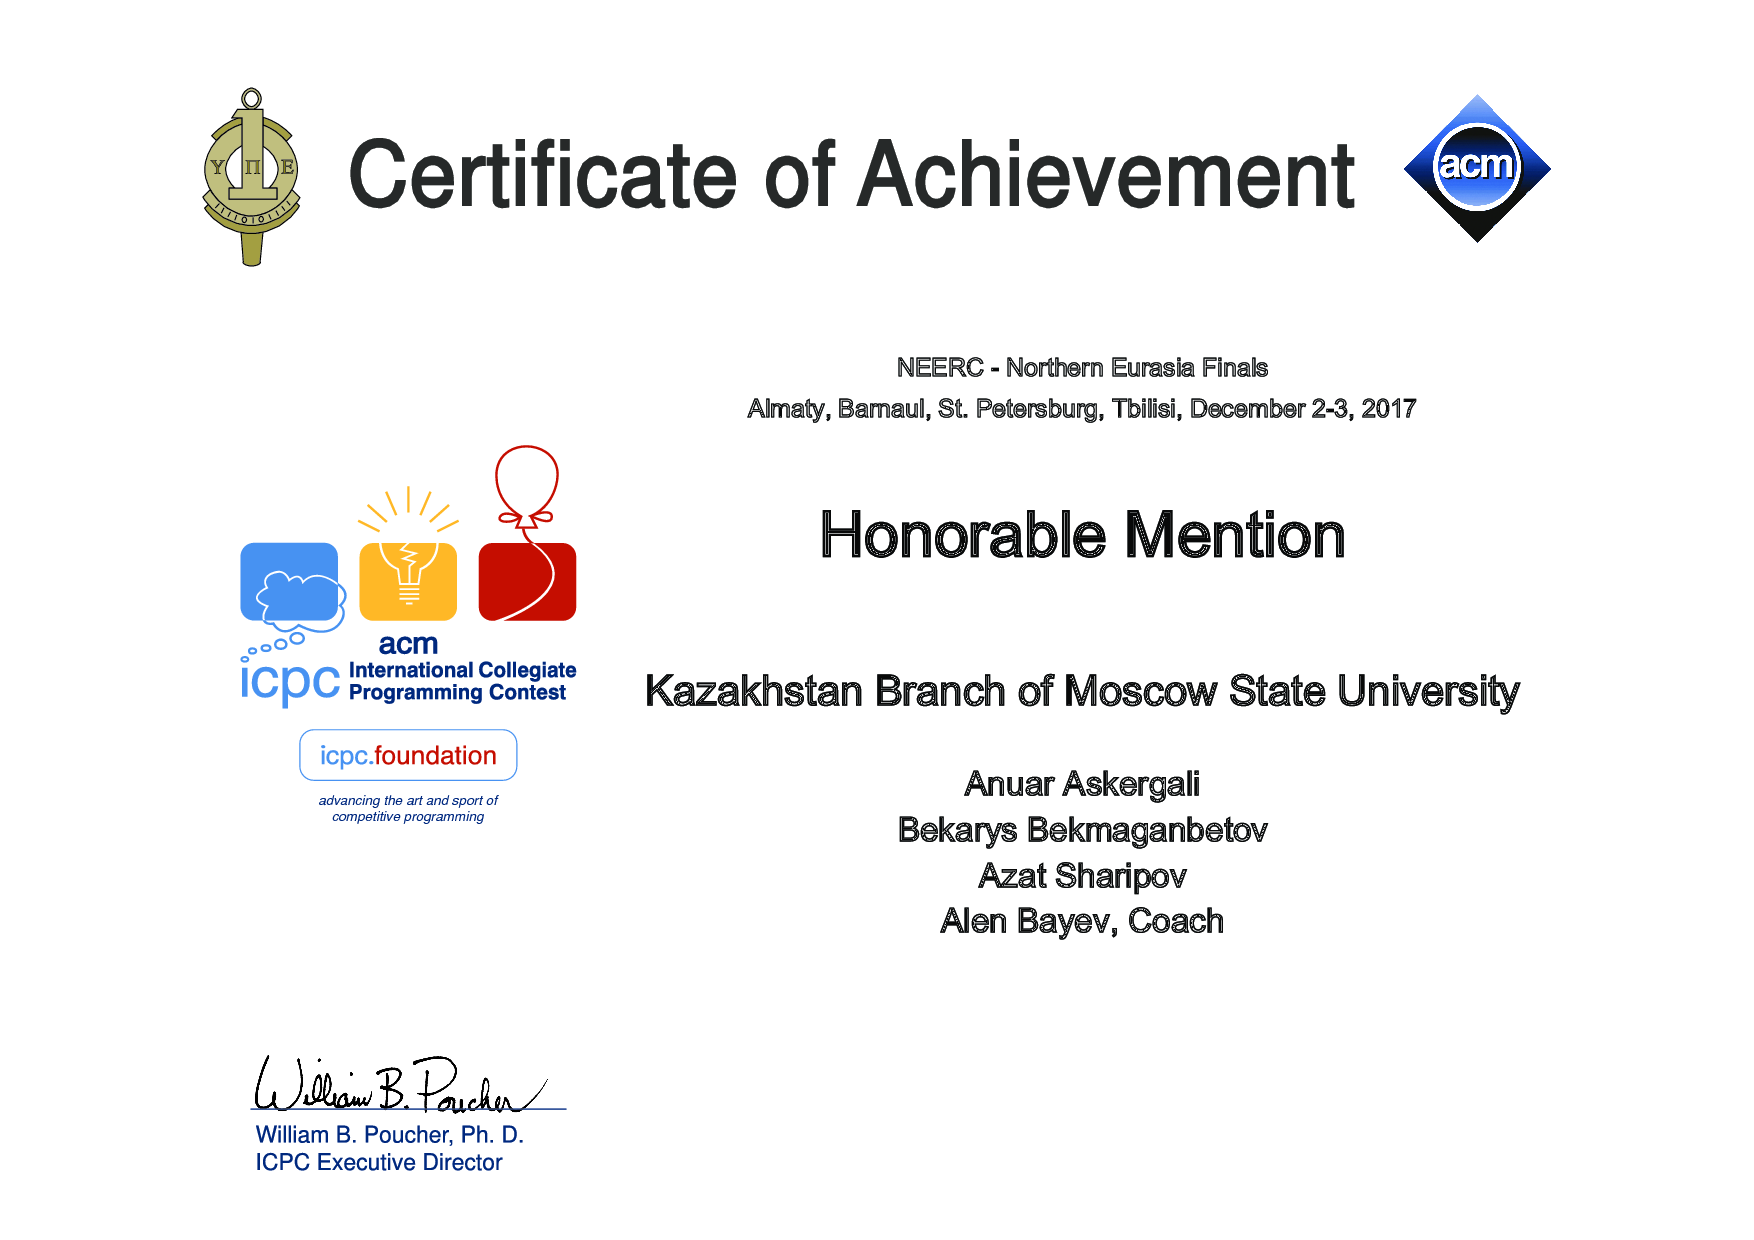
\includegraphics[width=0.9\linewidth]{diploma/2017-almaty}

Похвальная грамота среди команд Северо-Восточного европейского региона (СНГ).

Команда Brain Burst (Аскергалиев, Бекмаганбетов, Шарипов).
\end{center}
\vfill
\mbox{}
\newpage

